\documentclass[12pt]{article}
\usepackage{graphicx}
\addtolength{\oddsidemargin}{-.875in}
\addtolength{\evensidemargin}{-.875in}
\addtolength{\textwidth}{1.75in}
\addtolength{\topmargin}{-.875in}
\addtolength{\textheight}{1.75in}
\begin{document}

\noindent \emph {Fourth Development Sprint Memo}

\hfill April 24th, 2017

\noindent \textbf {To} \hspace{32pt}Bruce Bolden

\noindent \textbf {From} \hspace{16pt}Andrew Butler

\noindent \textbf {Subject} \hspace{4pt}Fourth Development Sprint Report

\section*{Introduction}

\hspace{14pt}This is the report detailing my efforts during the fourth and final development sprint of our team project, as well as providing a summary of my experience with the project as a whole.

\section*{Overview}

\hspace{14pt}This sprint I was primarily responsible for adding a "box select" feature. If the user holds shift when clicking a Node, the box bounded by this Node and the last Node clicked will be filled with the current color. I was also tasked with fixing a few bugs.
\section*{Summary}

\hspace{14pt} In order to add this feature, I needed figure out how to detect when shift was pressed while a click event was triggered. Luckily, Java provides a simple method for this. I added this check to the event listener for our Node buttons, then made a call to a function that would fill the rectangle of Nodes. This method accepts the following arguments: the currently selected Color, and integers for the minimum row, minimum column, maximum row, and maximum column to be filled. To calculate the maximum and minimum values, the previously clicked Node's location is always saved, and then used if a Node is clicked while shift is pressed. In addition to implementing this feature, I also fixed several bugs. The right click context menu on the Frame previews wasn't showing up on Unix based systems. To fix this, I needed to add checks in both the mousePressed and mouseReleased methods of the MouseListener for these Frame previews. I also made a fix to the behavior of the program on startup. Previously, clicking a Node immediately after starting the program would have no effect, the user would have to click a Frame preview first. I added a call to the button listener generation method on startup and when loading a file. Finally, I removed some redundant code, and commented out the menu options that are not going to be implemented before the end of this project. 
\linebreak

Overrall, my experience creating this project was a very positive one. I enjoyed working with my team, practicing Java, and learning more about the software development cycle. Future work on this program could include redesigning the color chooser to be more visually appealing, implementing a way to reorder frames, and adding a feature that would convert images or even videos to Frames and/or .tan files.

\pagebreak

\section*{Appendix A}

\begin{figure}[h]
  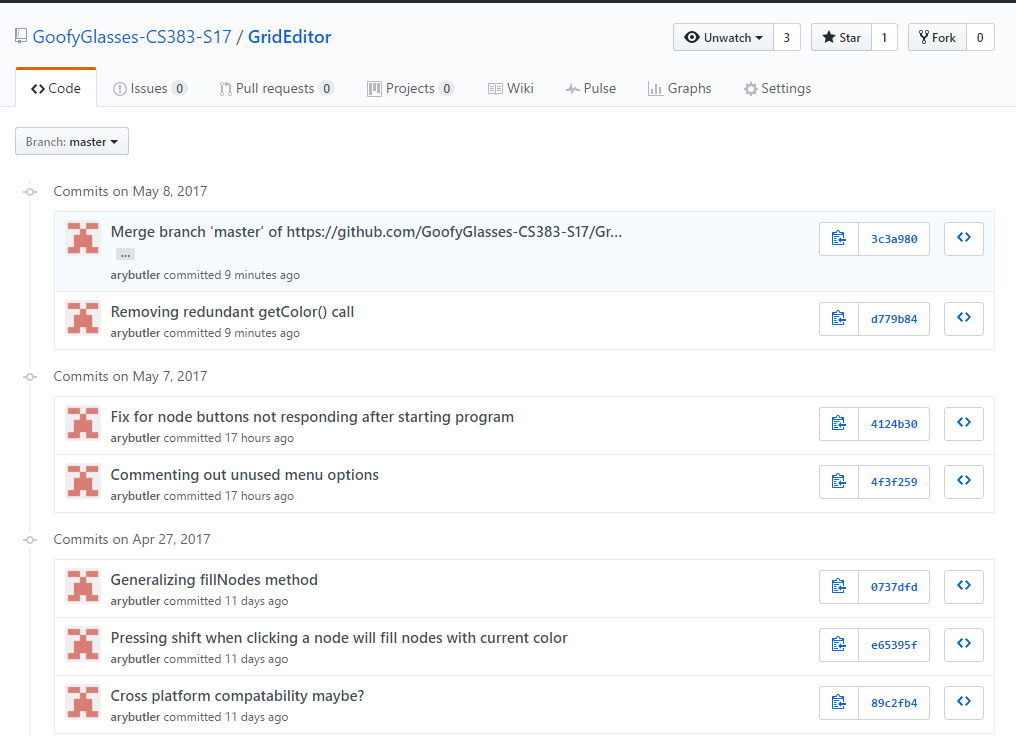
\includegraphics[width=\linewidth]{Commits.png}
  \caption{Most of my commits to the GitHub repository.}
  \label{fig:Git commits}
\end{figure}


\begin{figure}[h]
  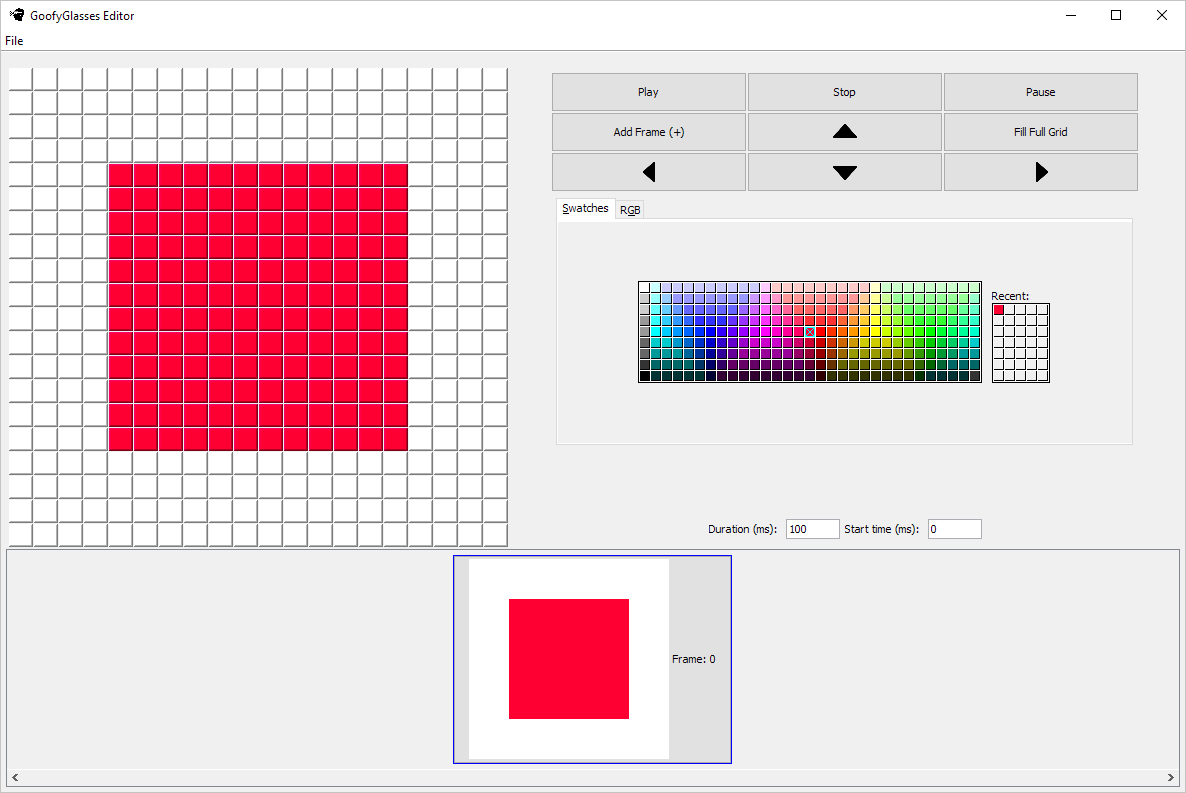
\includegraphics[width=\linewidth]{GUI.png}
  \caption{A box created with the shift-select feature.}
  \label{fig:Git commits}
\end{figure}

\end{document}